\documentclass[11pt]{article}

\usepackage[T1]{fontenc}
\usepackage[utf8]{inputenc}
\usepackage{lmodern}
\usepackage[margin=1in]{geometry}
\usepackage{amsmath}
\usepackage{booktabs}
\usepackage{graphicx}
\usepackage[numbers,sort&compress]{natbib}
\usepackage{xcolor}
\usepackage[colorlinks=true,linkcolor=blue!50!black,citecolor=blue!50!black,urlcolor=blue!50!black]{hyperref}
\usepackage{microtype}
\usepackage{caption}
\usepackage{enumitem}
\usepackage{tikz}
\usetikzlibrary{positioning,arrows.meta}

\setlist{nosep,leftmargin=1.4em}
\captionsetup{font=small,labelfont=bf}

% TODO(author): full name and affiliation.
\newcommand{\authorname}{Vincent}

\title{Confidence Is Not Groundedness:\\Calibrated Abstention for Claim Verification,\\from FEVER to YouTube Captions}
\author{\authorname}
\date{October 2026}

\begin{document}
\maketitle

\begin{abstract}
Claim-verification systems are usually compared by accuracy, but a checker that shows verdicts to
readers must also know when not to answer. We study calibrated abstention for evidence-based claim
verification on FEVER, then carry it into a local browser extension that checks claims in YouTube
captions against live news. On FEVER, vector scaling fitted on a separate calibration split reduces
expected calibration error from 0.129 to 0.031, and a confidence band promised at 90\% accuracy on that
split delivers 92.1\% on 31\% of test claims. Confidence, however, barely registers whether the model
was given the evidence it needed: on claims whose gold evidence never reached the model, mean confidence
is only 0.037 lower. A retrieval-side sufficiency score predicts that condition far better (AUC 0.75
against 0.59) but barely predicts correctness (0.53), so we use it as a second gate rather than blending
it into confidence. The gated system declines 44\% of ungrounded claims against 18\% of grounded ones,
at a cost of 18 points of coverage. Relabelling ungrounded training rows as not-enough-evidence lowers
NEI F1 by 0.07; dropping them costs nothing overall. Out of domain, a sentence-level judge is wrong on 10
of the 18 news sentences it counts, yet fixed composition rules that abstain by default point the right
way on 42 of 45 directional readings in a pre-registered batch of 142 claims. Real captions are a
different matter: in seven checks of political speeches, five of the six directional readings rested on a
reprint of the speech itself, and two of the three that could be scored were wrong.
\end{abstract}

\section{Introduction}

An automated fact-checking pipeline detects a claim, retrieves evidence and predicts a verdict
\citep{guo2022survey}. Benchmarks such as FEVER \citep{thorne2018fever} score the verdict by accuracy.
A checker that sits beside a video is used differently: a viewer reads its verdict without seeing what
it failed to retrieve, so its most damaging error is a confident verdict resting on evidence that does
not address the claim. The relevant framework is selective prediction \citep{elyaniv2010selective,
geifman2017selective}, where a model answers only when it is likely to be right and abstains otherwise.

Selective prediction rests on the model's confidence. FEVER makes that a hard test, because its claims
carry artifacts that let a model predict the label without reading any evidence
\citep{schuster2019debiasing}. When a model can be right without evidence, being right and having the
evidence come apart, and confidence may track the first but not the second. We ask whether a verifier's
confidence knows if it was given the evidence it needed, and if not, what does. The paper makes four
contributions:
\begin{itemize}
  \item A calibration and selective-prediction study of a retrieved-evidence DeBERTa verifier on FEVER,
        with every threshold frozen on a calibration split before test is read, and a target that the
        test split missed reported as missed (\S\ref{sec:calibration}).
  \item Evidence that confidence barely tracks groundedness, that a retrieval-side sufficiency model
        tracks it much better but not correctness, and that blending the two into one score degrades the
        ranking, so we use them as separate conditions (\S\ref{sec:groundedness}).
  \item A training-signal intervention that separates two effects of regrounding: dropping ungrounded
        rows costs nothing overall, relabelling them as not-enough-evidence damages the class it was meant
        to teach (\S\ref{sec:training}).
  \item A transfer of these principles to claims in live video, where a sentence-level judge is measured
        on news, verdicts are composed by fixed rules that abstain by default, and the end-to-end result is
        measured on batches of claims written before retrieval, one of them registered in advance, and on a
        small set of real-caption checks, including where it fails (\S\ref{sec:video}).
\end{itemize}

\section{Related Work}

\paragraph{Fact verification and its artifacts.} FEVER \citep{thorne2018fever} pairs Wikipedia-derived
claims with sentence-level evidence. Claim-only models perform well above chance on it
\citep{schuster2019debiasing}, as hypothesis-only models do on NLI \citep{gururangan2018artifacts}.
AVeriTeC \citep{schlichtkrull2023averitec} collects real-world claims with web evidence. Atanasova et al.\
\citep{atanasova2022insufficient} study how verifiers behave when evidence is removed, which is close to
our question of whether confidence registers missing evidence.

\paragraph{Calibration and selective prediction.} Temperature and vector scaling \citep{guo2017calibration}
and isotonic regression \citep{zadrozny2002multiclass} are standard post-hoc calibrators; pre-trained
transformers are reasonably calibrated in domain but less so out of it \citep{desai2020calibration}. We
report expected calibration error \citep{naeini2015ece}, the Brier score \citep{brier1950verification},
and the excess area under the risk--coverage curve, E-AURC \citep{geifman2019bias}. Kamath et al.\
\citep{kamath2020selective} show that a calibrator trained to predict correctness improves selective
question answering under domain shift; our sufficiency gate is related but predicts groundedness, a
different target.

\paragraph{Check-worthiness.} ClaimBuster \citep{hassan2017claimbuster, arslan2020benchmark} provides
sentence-level check-worthiness labels from US presidential debates, which we use to train the detector
that selects claims from captions.

\section{Setup on FEVER}
\label{sec:setup}

\paragraph{Data and splits.} Models are trained on the FEVER training set. The released development set is
split in half by a hash of the claim, stratified by label, into a calibration half and a test half.
Experiments use 2,000-claim samples of each (test: 682 supported, 668 refuted, 650 not enough evidence,
NEI). Every calibrator, band threshold and gate threshold is fitted on the calibration sample. The test
half is not FEVER's hidden test set. A separate holdout of about 5,000 training claims is used for model
selection and to fit the sufficiency model itself.

\paragraph{Retrieval.} BM25 \citep{robertson2009bm25} over 5,416,536 Wikipedia pages retrieves 25 pages,
with up to three further pages whose titles appear in the claim, and their sentences are ranked into a
25-sentence budget. Strict recall@25, a complete gold evidence group among the 25 sentences, is 0.811 on
verifiable test claims (0.801 on calibration). Document recall at 25 pages is 0.896, so of the 18.9 points
lost on the way to 0.811, 10.4 are lost finding pages and 8.5 selecting sentences from them.

\paragraph{Verdict model.} DeBERTa-v3-base \citep{he2023debertav3} reads the claim and the evidence packed
into 512 tokens, and predicts supported, refuted or NEI. Three variants share the architecture:
\emph{claim-only} (no evidence), \emph{retrieved} (the system) and \emph{gold} (gold evidence, an oracle).
NEI claims have no gold evidence, so the retrieved and gold variants receive byte-identical inputs on them:
evidence count and token length agree on all 650 NEI test claims.

\paragraph{Groundedness.} A verifiable claim is \emph{gold read} when a complete gold group survives into
the packed input, and \emph{gold missed} otherwise. After packing, 77.4\% of verifiable test claims are gold
read (1,045 of 1,350); this is the packed retrieval ceiling quoted beside verdict accuracy.

\section{Results on FEVER}

\subsection{Evidence and the claim-only baseline}

\begin{table}[t]
\centering
\small
\begin{tabular}{lccc}
\toprule
Variant & Accuracy & Macro F1 & NEI recall \\
\midrule
Majority class & 0.341 & -- & -- \\
Claim only & 0.587 & 0.565 & 0.302 \\
Retrieved & 0.702 & 0.690 & 0.475 \\
Gold (oracle) & 0.878 & 0.878 & 0.860 \\
\bottomrule
\end{tabular}
\caption{Uncalibrated verdict accuracy on 2,000 test claims. Retrieved evidence adds 0.115 over
claim-only (paired bootstrap 95\% CI [0.096, 0.135], McNemar \citep{mcnemar1947} $p = 6.4\times10^{-30}$);
gold evidence adds a further 0.176 [0.157, 0.196].}
\label{tab:variants}
\end{table}

Table~\ref{tab:variants} shows that evidence matters and that FEVER's artifact is large: without evidence
the model reaches 0.587 against a 0.341 majority class, and it is right on 72.4\% of verifiable claims.
The NEI column is the informative one. On NEI claims the retrieved and gold variants see identical inputs,
yet the retrieved model recalls NEI 47.5\% of the time against the gold model's 86.0\%, and 252 of its 341
NEI errors are predictions of supported. Since the inputs are identical, the difference comes from what
each model learned in training. One plausible contributor is that a model trained on retrieved evidence
regularly sees verifiable claims whose gold evidence was never retrieved, labelled supported or refuted
anyway, so missing evidence stops implying NEI. Removing those rows from training does not recover NEI
recall, however (\S\ref{sec:training}), so they do not explain the gap on their own.

\subsection{Calibration and selective prediction}
\label{sec:calibration}

We compare temperature scaling, isotonic regression and vector scaling in a restricted form, a single
temperature with a per-class bias (Guo et al.'s version scales each class separately), by five-fold
out-of-fold negative log-likelihood on the calibration split. Vector scaling wins for all three variants
(retrieved: 0.673, against 0.728 for temperature, 0.728 for isotonic and 0.823 uncalibrated).
Table~\ref{tab:calibration} reports the result on test.

\begin{table}[t]
\centering
\small
\begin{tabular}{lcc}
\toprule
Retrieved variant, test & Uncalibrated & Vector scaling \\
\midrule
Accuracy & 0.702 & 0.729 \\
ECE (15 bins) & 0.129 [0.108, 0.147] & 0.031 [0.026, 0.054] \\
Maximum calibration error & 0.152 & 0.057 \\
Brier score & 0.441 & 0.374 \\
NLL & 0.812 & 0.647 \\
NEI F1 & 0.573 & 0.646 \\
\bottomrule
\end{tabular}
\caption{Calibration fitted on the calibration split, measured on test. The Brier change is $-0.067$
[$-0.080$, $-0.054$], paired. Accuracy changes because the per-class bias moves the argmax. Calibrated
ECE is 0.034 for claim-only and 0.018 for gold.}
\label{tab:calibration}
\end{table}

Because the calibrator includes a per-class bias, it corrects the model's prior shift toward supported as
well as its overconfidence. Accuracy rises by 2.7 points and NEI F1 by 7.4, the largest change in the
weakest cell. Figure~\ref{fig:calibration} shows the reliability diagrams and the risk--coverage curve.

\begin{figure}[t]
\centering
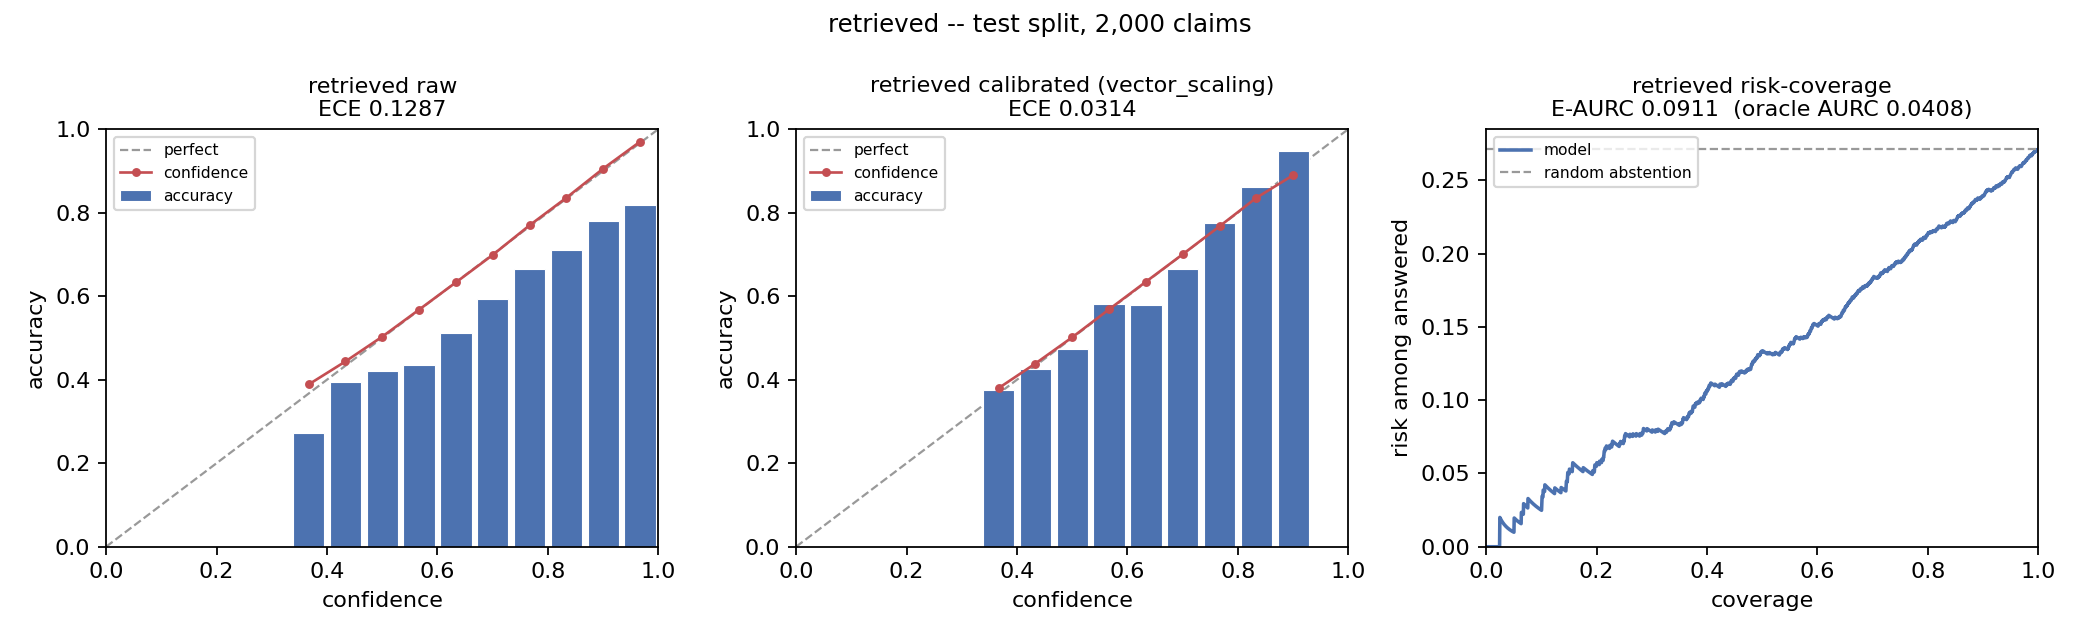
\includegraphics[width=\linewidth]{figures/calibration_retrieved.png}
\caption{Retrieved variant on 2,000 test claims: reliability before and after vector scaling, and the
risk--coverage curve after calibration (E-AURC 0.091; AURC 0.132 against an oracle 0.041).}
\label{fig:calibration}
\end{figure}

For abstention, three confidence bands are fitted on out-of-fold calibrated probabilities on the
calibration split, with accuracy targets of 0.90, 0.75 and 0.60 stated in advance; claims below the weakest
band receive no verdict. On test, the strong band delivers 0.921 on 618 claims (31\% of test) and the
moderate band 0.789 on 479. The weak band delivers 0.594 on 715 against its 0.60 target, a miss of 0.006,
which we report rather than refit. The system abstains on 9.4\% of claims. On the test risk--coverage
curve, 90\% accuracy is reachable at 38.8\% coverage and 95\% at 19.3\%. The band boundaries are sensitive
to the fit: rerunning the same procedure with a different cross-fitting seed moves test coverage from 0.906
to 0.936 (Table~\ref{tab:abstention}).

\subsection{Confidence barely tracks groundedness}
\label{sec:groundedness}

\begin{table}[t]
\centering
\small
\setlength{\tabcolsep}{5pt}
\begin{tabular}{lcccccc}
\toprule
& & Answered & \multicolumn{3}{c}{Declined when \ldots} & Share gold \\
\cmidrule(lr){4-6}
Policy (test) & Coverage & accuracy & gold missed & gold read & NEI & missed$^{*}$ \\
\midrule
Bands of \S\ref{sec:calibration} (seed 0) & 0.906 & 0.757 & 11.5\% & 7.6\% & 11.4\% & 30.7\% \\
Refitted bands (seed 42) & 0.936 & 0.751 & 8.9\% & 5.5\% & 6.9\% & 32.1\% \\
\quad + sufficiency $\geq 0.5$ & 0.758 & 0.755 & 43.9\% & 18.1\% & 24.8\% & 41.5\% \\
\bottomrule
\end{tabular}
\caption{Which claims each abstention policy declines. The test split has 305 gold-missed, 1,045 gold-read
and 650 NEI claims; 22.6\% of verifiable claims are gold missed. $^{*}$Gold-missed claims as a share of the
declined verifiable claims, comparable with that 22.6\%. The first two rows differ only in the
cross-fitting seed used to place the bands; the last two only in the sufficiency condition.}
\label{tab:abstention}
\end{table}

On test, the calibrated retrieved model is right on 79.9\% of gold-read claims and 72.5\% of gold-missed
ones, but its mean confidence differs by only 0.037 between the two (0.752 against 0.715). It still answers
most ungrounded claims correctly (on the calibration split, 65.4\% of the 298 gold-missed claims), which
the claim-only results suggest it does from the claim's wording, so there is little reason for its
confidence to fall on them. A logistic model fitted on the verdict logits predicts whether the gold
evidence was read with an AUC of only 0.586 on verifiable calibration claims.

Table~\ref{tab:abstention} shows the consequence. Confidence-based abstention does prefer ungrounded claims,
but weakly: the bands of \S\ref{sec:calibration} decline 11.5\% of gold-missed claims and 7.6\% of gold-read
ones, a ratio of 1.5. Residual overconfidence after calibration is largest on NEI claims, where mean
confidence exceeds accuracy by 0.066 (0.026 on refuted claims; supported claims are underconfident).

\paragraph{A sufficiency signal.} We fit a logistic regression on eleven features of the BM25 score
distribution (top, mean and minimum score, spread, decay, margin and ratio, the number of distinct pages,
the top page's share, where the first page change occurs and how many sentences were read), trained to
predict gold read on 3,510 verifiable holdout claims. On verifiable calibration claims it predicts gold
read with AUC 0.748, against 0.586 for the verdict logits, and adding the logits does not help (0.748).
It says little about correctness: on all 2,000 calibration claims, with out-of-fold calibrated confidence,
it predicts correctness with AUC 0.531 against 0.717 for confidence, and the two scores correlate at 0.03.
Multiplying them degrades the correctness ranking (E-AURC 0.114 to 0.149). Groundedness and correctness
are different targets on FEVER, consistent with the claim-only artifact.

We therefore gate on both conditions separately: answer only when a confidence band is assigned
\emph{and} predicted sufficiency is at least 0.5, the model's own decision boundary rather than a tuned
value. The gate declines 43.9\% of gold-missed claims against 18.1\% of gold-read ones, a ratio of 2.4,
and gold-missed claims rise from 32.1\% to 41.5\% of the declined verifiable claims. Accuracy on answered
claims barely moves (0.751 to 0.755) while coverage falls from 0.936 to 0.758: honest abstention is bought
with coverage, not accuracy.

\subsection{The training signal}
\label{sec:training}

On the training split, 29,309 of 106,297 verifiable rows (27.6\%) are ungrounded: their retrieved evidence
does not contain a complete gold group, yet they carry a supported or refuted label. Regrounding them does
two things at once, removing contradictory supervision and teaching NEI on ungrounded input, so we train
two arms with the same recipe and calibrate each on the calibration split (Table~\ref{tab:training}).

\begin{table}[t]
\centering
\small
\begin{tabular}{lccc}
\toprule
Test, calibrated & Control & Dropped & Relabelled NEI \\
\midrule
Accuracy, gold read (1,045) & 0.799 & 0.822 & 0.833 \\
Accuracy, gold missed (305) & 0.725 & 0.613 & 0.400 \\
Accuracy, NEI claims (650) & 0.617 & 0.623 & 0.571 \\
NEI F1 & 0.646 & 0.646 & 0.575 \\
NEI predictions (650 true NEI) & 591 & 603 & 641 \\
Accuracy overall & 0.729 & 0.726 & 0.682 \\
\quad paired change vs control & -- & $-0.003$ [$-0.017$, $0.011$] & $-0.047$ [$-0.067$, $-0.028$] \\
\quad McNemar $p$ & -- & 0.73 & $2.8\times10^{-6}$ \\
Corr(confidence, sufficiency) & 0.090 & 0.009 & 0.033 \\
\bottomrule
\end{tabular}
\caption{Training on all rows (control), dropping the 29,309 ungrounded rows, or relabelling them NEI,
all on 2,000 test claims.}
\label{tab:training}
\end{table}

Dropping the ungrounded rows raises accuracy on gold-read claims by 2.3 points, leaves NEI F1 unchanged
and costs nothing overall; accuracy on gold-missed claims falls, as it should once the model no longer
learns to answer without evidence. Relabelling them NEI was predicted to raise NEI F1 and instead lowers it
by 0.072: the model predicts NEI more often while identifying true NEI worse, because the extra predictions
land on gold-missed verifiable claims, which is what it was trained to do. Relabelling declares \emph{I was
not given the evidence} and \emph{there is no evidence} to be the same case, so the model treats them as
the same case. Neither arm made confidence track sufficiency on test.

\subsection{External validity}

Whether these findings are specific to FEVER could not be settled with AVeriTeC
\citep{schlichtkrull2023averitec} at this model scale. AVeriTeC's labelled release has 3,568 claims. We ran
one size-matched comparison, about 2,100 training claims with the MIXED class dropped to give three classes:
the FEVER verifier predicted the majority class for every test claim, while the AVeriTeC verifier scored a
few points above its majority class on about 500 test claims.\footnote{These two runs' outputs were not
retained locally, so their values come from the project's run log.} A unigram naive Bayes probe at 2,556
training claims shows similar claim-only lifts over the majority class on both (+0.068 on three-class FEVER,
+0.063 on four-class AVeriTeC). At the one matched size we ran, one model is degenerate, so the comparison
is not identified, and we draw no conclusion about AVeriTeC's artifacts.

\section{Claims in Live Video}
\label{sec:video}

\begin{figure}[t]
\centering
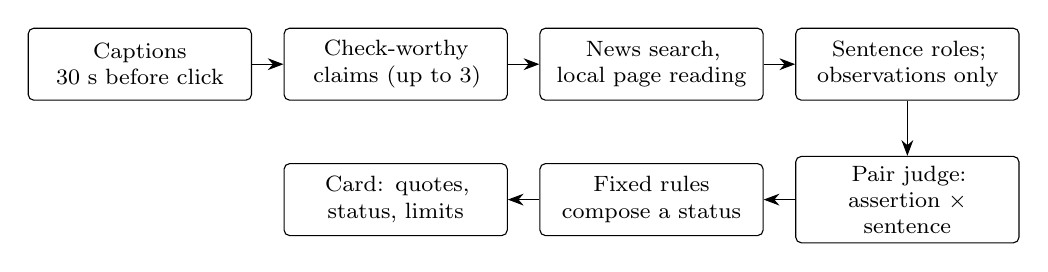
\begin{tikzpicture}[
  box/.style={draw, rounded corners=2pt, align=center, font=\footnotesize, minimum height=2.6em, text width=7.4em},
  arr/.style={-{Stealth[length=2mm]}}]
\node[box] (cap) {Captions\\30 s before click};
\node[box, right=0.4cm of cap] (det) {Check-worthy\\claims (up to 3)};
\node[box, right=0.4cm of det] (ret) {News search,\\local page reading};
\node[box, right=0.4cm of ret] (role) {Sentence roles;\\observations only};
\node[box, below=0.7cm of role] (judge) {Pair judge:\\assertion $\times$ sentence};
\node[box, left=0.4cm of judge] (comp) {Fixed rules\\compose a status};
\node[box, left=0.4cm of comp] (card) {Card: quotes,\\status, limits};
\draw[arr] (cap) -- (det); \draw[arr] (det) -- (ret); \draw[arr] (ret) -- (role);
\draw[arr] (role) -- (judge); \draw[arr] (judge) -- (comp); \draw[arr] (comp) -- (card);
\end{tikzpicture}
\caption{The check behind each click. Everything runs on the viewer's machine except the news search and
page fetches. No model writes the conclusion.}
\label{fig:pipeline}
\end{figure}

The FEVER verifier is out of domain on political speech, and a June 2017 Wikipedia cannot establish recent
events. The demonstration system (Figure~\ref{fig:pipeline}) is a browser extension that reads YouTube's
caption data, without turning on captions, and passes the 30 seconds before the viewer's click to a local
Python process. A DeBERTa detector trained on ClaimBuster \citep{arslan2020benchmark} picks the most recent
check-worthy sentences; on 120 sentences from the 2016 State of the Union, labelled by the author, it
reaches F1 0.792 against 0.310 for the hand-written rules it replaced, although the labels and the rules
share an author. Evidence comes from Google News search and the pages it links to, read locally.

\subsection{Decomposed judgment}

Every local language model we tried as a writer of the verdict misread news evidence in the same ways:
opinions promoted to proof, worked examples read as measurements, definitions and populations changed in
paraphrase. The failure was the same across the models we tried, so we changed the task rather than the
model. Each claim is split into assertions (a contrast becomes two). Each source sentence gets an exact
span identity, and closed-class cues type it as opinion, forecast, illustration, definition, navigation or
image caption; only reported observations are eligible to count. A pair judge, DeBERTa-v3-base with four
outputs (states, states the negation, bears on, unrelated), is trained on pairs derived from FEVER and MNLI
\citep{williams2018mnli}; a negated assertion is judged in its positive form and the answer inverted. On
held-out FEVER/MNLI pairs it reaches 0.886 accuracy, and a counting band fitted to a 5\% counting-error
target keeps 69.1\% of counts at 5.1\%, a narrow miss.

Composition is a fixed set of rules, with abstention as the default:
\begin{itemize}
  \item Only \emph{states} and \emph{states the negation} judgments inside the counting band, on eligible
        sentences from pages found by searching for the claim (not by a separate search for its terms),
        can count. \emph{Bears on} is shown and never counts.
  \item A stated period wholly outside the claim's demotes a count to context. A narrower place in the
        sentence (a state or province of the claim's country) or a quantified group such as ``several
        states'' leaves the count standing but makes the assertion qualified, never established.
  \item A page read both as stating and as denying an assertion is a misreading, and none of its counts count.
  \item An assertion is established by an unqualified count from one independent source with a confirmed
        publication date, when the claim's country is known; a linked page or a second page on one publisher
        is the same source. Anything less is reported as qualified, and opposing sources make it contested.
  \item A contrast is established only when every one of its assertions is.
\end{itemize}
The card quotes the counted and bearing sentences verbatim with their sources, says how each was read, and
names every limit; nothing is paraphrased. These are the current rules. Each batch below is scored on the
result recorded when it was run, under the rules in force then: the self-conflict and quantified-group rules
came after the probe batch, the single-source rule after the first two batches, and the image-caption cue
after the held-out batch.

\subsection{The sentence judge on news}

To measure the judge on news, 36 claims across economics, crime, health, demographics and trade in nine
countries were written before any source was seen, then checked through the host with the country declared.
Their 1,060 (assertion, sentence) pairs were labelled by a language-model annotator blind to the judge's
output. At the shipped counting threshold, the judge counted 18 sentences and 10 were wrong, a counting
error of 0.56 (95\% Wilson interval [0.34, 0.75]); no threshold in the sweep reached the 5\% target. Read
back, most of the errors are scope and comparison errors: a state's figure counted for the country, a
2020-to-2024 change counted for ``fell in 2024'', a dairy surplus read as denying an overall trade
deficit. One was a campaign promise read as a denial.

Two news-adapted retrains were judged by a rule fixed before training: at most 25\% counting error with at
least 12 counts on these probe labels, and held-out FEVER/MNLI accuracy within one point. Adding 2,274
labelled news pairs gave 15 wrong of 22 counts. A second batch of 117 claims was written so that retrieval
would surface sentences stating or denying them; adding the labelled pairs of 76 of those claims to the
same news pairs gave 7 wrong of 14, and on the remaining 41 claims (1,065 pairs, never trained on) 20 wrong
of 46 against the original judge's 24 of 45. Neither met the rule, and the original judge remains in use.

\subsection{End to end: direction of the composed reading}

We score the product's composed reading, not the judge. An assertion's reading is \emph{directional} when
its status points for the claim (supported or qualified support) or against it (contradicted or qualified
contradiction), and a directional reading is right when it agrees with the claim's truth value. Contested
readings point both ways and are not scored.

\begin{table}[t]
\centering
\small
\begin{tabular}{lcccc}
\toprule
Batch & Claims & Directional & Right & Established \\
\midrule
Probe and count batches (decision made on these) & 153 & 47 & 47 & 5 \\
Held-out batch, registered before clicking & 142 & 45 (31.7\%) & 42 (93.3\%) & 35 \\
Real captions, author's truth values & 17 & 3 scored & 1 & 3 \\
\bottomrule
\end{tabular}
\caption{Direction of the composed reading. All claims in the first two rows were written as single
sentences by a language-model annotator. The count batch's truth values are those its claims were written
under (true, or deliberately altered); the probe batch's were recorded by the same annotator after the
clicks, having seen which claims received a direction. Only the held-out batch was registered, claims,
truth-file hash and decision rule, before it was run. ``Established'' follows the rules in force when each
batch was recorded: two independent sources for the first row, one dated source after. Real-caption claims
come from seven checks on four videos; the author left seven claims unsettled, three of which received a
directional reading.}
\label{tab:directions}
\end{table}

Table~\ref{tab:directions} contains the main out-of-domain result. On the first two batches, 153 claims,
the composed reading pointed a direction 47 times and was right every time, while the sentence judge beneath
it counted wrongly about half the time. Our reading of the records, not a measured quantity, is that a wrong
count usually lands on a page that is about the claim being true or false, so it often points the right way,
and the rules hold back many of the rest. On that measurement the original requirement of two independent
sources was relaxed to one dated source, and the decision was tested on a new batch of 142 claims whose
truth values were fixed and hashed before it was run: 42 of 45 directional readings were right (Wilson 95\%
interval [0.82, 0.98]) at 31.7\% coverage.

The errors are one-sided. Across both batches, readings for the claim were right 57 of 57 times and
readings against it 32 of 35. All three held-out errors are single-source contradictions of true claims,
each a sentence about a related event, or with a construction such as ``failed to'', read as a denial: a
photo caption about the president monitoring operations in Venezuela ``on Jan.~3'' read as denying
Maduro's capture; ``both leaders agreed to a trade war truce when they met \ldots\ in Busan'' read as
denying the Busan meeting; and ``Jan Suraaj Party failed to win even a single seat'' read as denying the
NDA's win. The image-caption cue was added after this measurement, on the first of these errors;
recomposed with it, the batch reads 41 of 43, which is in-sample for that cue. The card shows the quoted
sentence, so each error is checkable, but a single-source contradiction is where this system is least
reliable.

\paragraph{Real captions.} The batches above are clean, single-sentence claims written for the test.
Claims clicked in real videos are fragmentary, and a search for their exact words tends to return the
speech itself. We scored the seven checks recorded, outside the development video, before the author
filled in truth values: three presidential addresses and a vice-presidential debate. The author supplied
truth values for ten of the 17 researched claims; whether the cards were hidden while doing so was not
controlled. Six claims received a directional reading, and five of the six rested on a reprint of the
speech: a broadcaster's advance text or full transcript of the address, or an article quoting it. The
sixth rested on an unrelated sentence read as a denial. Three of the six could be scored. Two were false
claims read as supported, ``And over the past six years, illegal border crossings have been cut by more
than half,'' quoted in a 2026 article, and ``We suffered the worst inflation in 48 years,'' from the
broadcaster's transcript. The third was right only because the speaker was. No real-caption reading
rested on independent evidence. A source that reprints a claim is not evidence for it, but the role cues
that withhold transcripts and quoted speech recognised none of these sentences, and the clean batches were
unlikely to expose the failure. With $n = 3$ scored readings this is a failure mode, not an error rate.

\paragraph{Sufficiency out of domain.} On a random sample of 40 of the 84 State of the Union (2016) claims
that reached the verdict model, checked against the 2017 Wikipedia, the author labelled whether retrieval
returned anything that could bear on the claim. Only 14 of the 40 retrievals did. Sufficiency alone falls
below 0.5 for 30\% of these claims, against 19.1\% of FEVER test claims, and for 38\% of the irrelevant
retrievals against 14\% of the relevant ones. As a predictor of relevance its AUC is 0.58, with a 95\%
interval of [0.39, 0.75] that spans both chance and its FEVER value, so whether the gate transfers is
open; about ten times as many labels would settle it, and the scores were visible while labelling. Its
features describe the shape of the BM25 scores, which can look the same for the right page and for a
confident keyword match on the wrong one.

\section{Limitations}

\begin{itemize}
  \item \textbf{Annotation.} The news claims, their truth values and the 1,060 pair labels come from a single
        automated annotator, a language model; they are not human gold labels. The pair labels were made
        blind to the judge's answers, and the held-out truth values were fixed before that batch was run,
        but the probe batch's truth values were recorded after its clicks. The 120 check-worthiness
        sentences, the 40 relevance labels and the 17 real-caption truth values were labelled by the author,
        a single annotator.
  \item \textbf{Sample sizes.} The held-out end-to-end result rests on 45 directional readings and the
        real-caption result on three. The FEVER results use 2,000 test claims.
  \item \textbf{Retrieval.} News search results change from hour to hour, so the same click can read
        differently later. Retrieval often returns topically related but inapplicable sentences; ranking them
        well remains unsolved, and every attempt we made to filter them also removed useful evidence.
  \item \textbf{Development fit.} Most sentence role cues were chosen while reading one development video's
        sources; the opinion-section cue came from an earlier six-claim probe and the image-caption cue from
        the held-out batch. A misfiring cue withholds a sentence rather than counting it, which usually costs
        coverage, but withholding one side of a conflicting page can change a direction.
  \item \textbf{Scope.} The calibration, sufficiency and training findings are measured on FEVER. The one
        out-of-domain test of the sufficiency gate (40 claims) was inconclusive, and the AVeriTeC comparison
        could not be made at this scale.
\end{itemize}

\section{Conclusion}

On FEVER, post-hoc calibration makes a verifier's probabilities trustworthy enough to abstain on, but
confidence describes whether the answer is likely right, not whether the model was given the evidence, and
the two diverge wherever a claim's wording gives away its label. A retrieval-side signal recovers much of
the groundedness signal and works as a separate gate; teaching the distinction by relabelling erases it.
Moved to live news, the same principle, a narrow judge composed by rules that abstain unless the evidence
clears them, gave a reading that was rarely wrong on clean held-out claims but answered fewer than a third
of them. On real captions it met a failure the benchmarks never contain: the source was the speech itself.
Recognising reprints of the speaker's own words is the next fix this system needs. The code and
measurement scripts are in the project repository; \texttt{paper/PROVENANCE.md} there names the record and
command behind each number, and says which records are kept only locally or were not retained.

\bibliographystyle{plainnat}
\bibliography{references}

\end{document}
